%\documentclass[wsdraft]{ws-procs11x85}

\documentclass{ws-procs11x85}
\usepackage{ws-procs-thm}           % comment this line when `amsthm / theorem / ntheorem` package is used
\usepackage{amsmath}

\begin{document}

\title{A DISTRIBUTED INFRASTRUCTURE FOR DRUG EFFECT DISCOVERY USING SPONTANEOUS REPORTING SYSTEMS}

\author{RAMI S VANGURI}

\address{Department of Biomedical Informatics, Columbia University,\\
New York, NY 10032 USA\\
E-mail: r.vanguri@columbia.edu}

\author{JOSEPH D ROMANO}

\address{Department of Biomedical Informatics, Columbia University,\\
New York, NY 10032 USA\\
E-mail: jdr2160@columbia.edu}

\author{TAL LORBERBAUM}

\address{Department of Biomedical Informatics, Columbia University,\\
New York, NY 10032 USA\\
E-mail: tal.lorberbaum@columbia.edu}

\author{VICTOR NWANKWO}

\address{Department of Biomedical Informatics, Columbia University,\\
New York, NY 10032 USA\\
E-mail: vtn2106@columbia.edu}

\author{CHOONHAN YOUN}

\address{San Diego Supercomputer Center, University of California, San Diego,\\
La Jolla, CA 92093 USA\\
E-mail: cyoun@sdsc.edu}

\author{NICHOLAS P TATONETTI}

\address{Department of Biomedical Informatics, Columbia University,\\
New York, NY 10032 USA\\
E-mail: nick.tatonetti@columbia.edu}

\begin{abstract}
Adverse drug events are a leading cause of morbidity and mortality
around the world. Regulatory agencies, such as the Food and Drug
Administration (FDA), maintain large collections of adverse event
reports, providing an opportunity to retrospectively study drug and
drug combination effects.  We mined the FDA Adverse Event Reporting
System (FAERS) for significant adverse reactions and developed a
database of drug effects, known as nSides. FAERS contains millions of
reports covering thousands of drugs and thousands of effects,
requiring the computing of approximately X billion models. We present
a scalable, distributed, on-demand computational infrastructure which
can be used with spontaneous reporting systems to calculate side
effect significances from drug combinations. Even though nSides is
based on FAERS data, the presented infrastructure is portable can be
applied to any spontaneous reporting system.
\end{abstract}

% required
\bodymatter

\section{Introduction}

Spontaneous reporting systems such as the FDA Adverse Event Reporting
System (FAERS) and EudraVigilance are important resources for
detecting drug adverse events during and after the drug approval
process (pharmacovigilance). However, pharmacovigilance algorithms
often lead to many false positive and false negative findings due to
issues of confounding, and detection of drug-drug interactions is an
even greater challenge. When adverse reactions are caused by three or
more drugs taken simultaneously, the problem quickly becomes
computationally intractable. We previously developed databases for
off-label drug effects (O\textsc{ffsides}) and drug interactions
(T\textsc{wosides}) using FAERS that account for these limitations
using a novel Statistical Correction for Uncharacterized Bias
(SCRUB)~\cite{Tatonetti2012}.  We re-mined FAERS with an updated
algorithm to populate a new version of the databases, known as nSides.
nSides also contains a front-end component consisting of a web gateway
(http://nsides.io/) accessible to researchers, clinicians and patients
alike.

We present the computational infrastructure used to populate the
nSides back-end database, designed to be executed on grid computing
systems. Additionally, we present middleware used to communicate
between users and the back-end database.  The communication is done
via an on-demand interface where users can request the nSides back-end
database be populated with a specific drug combination. Drug
combinations must be calculated on an on-demand basis due to the very
high number of drug combinations possible in spontaneous reporting
systems. The goal is to populate the back-end database within 24 hours
of a user request. A diagram of the workflow is shown in
Fig.~\ref{fig:workflow}.

\begin{figure}[h]
\centerline{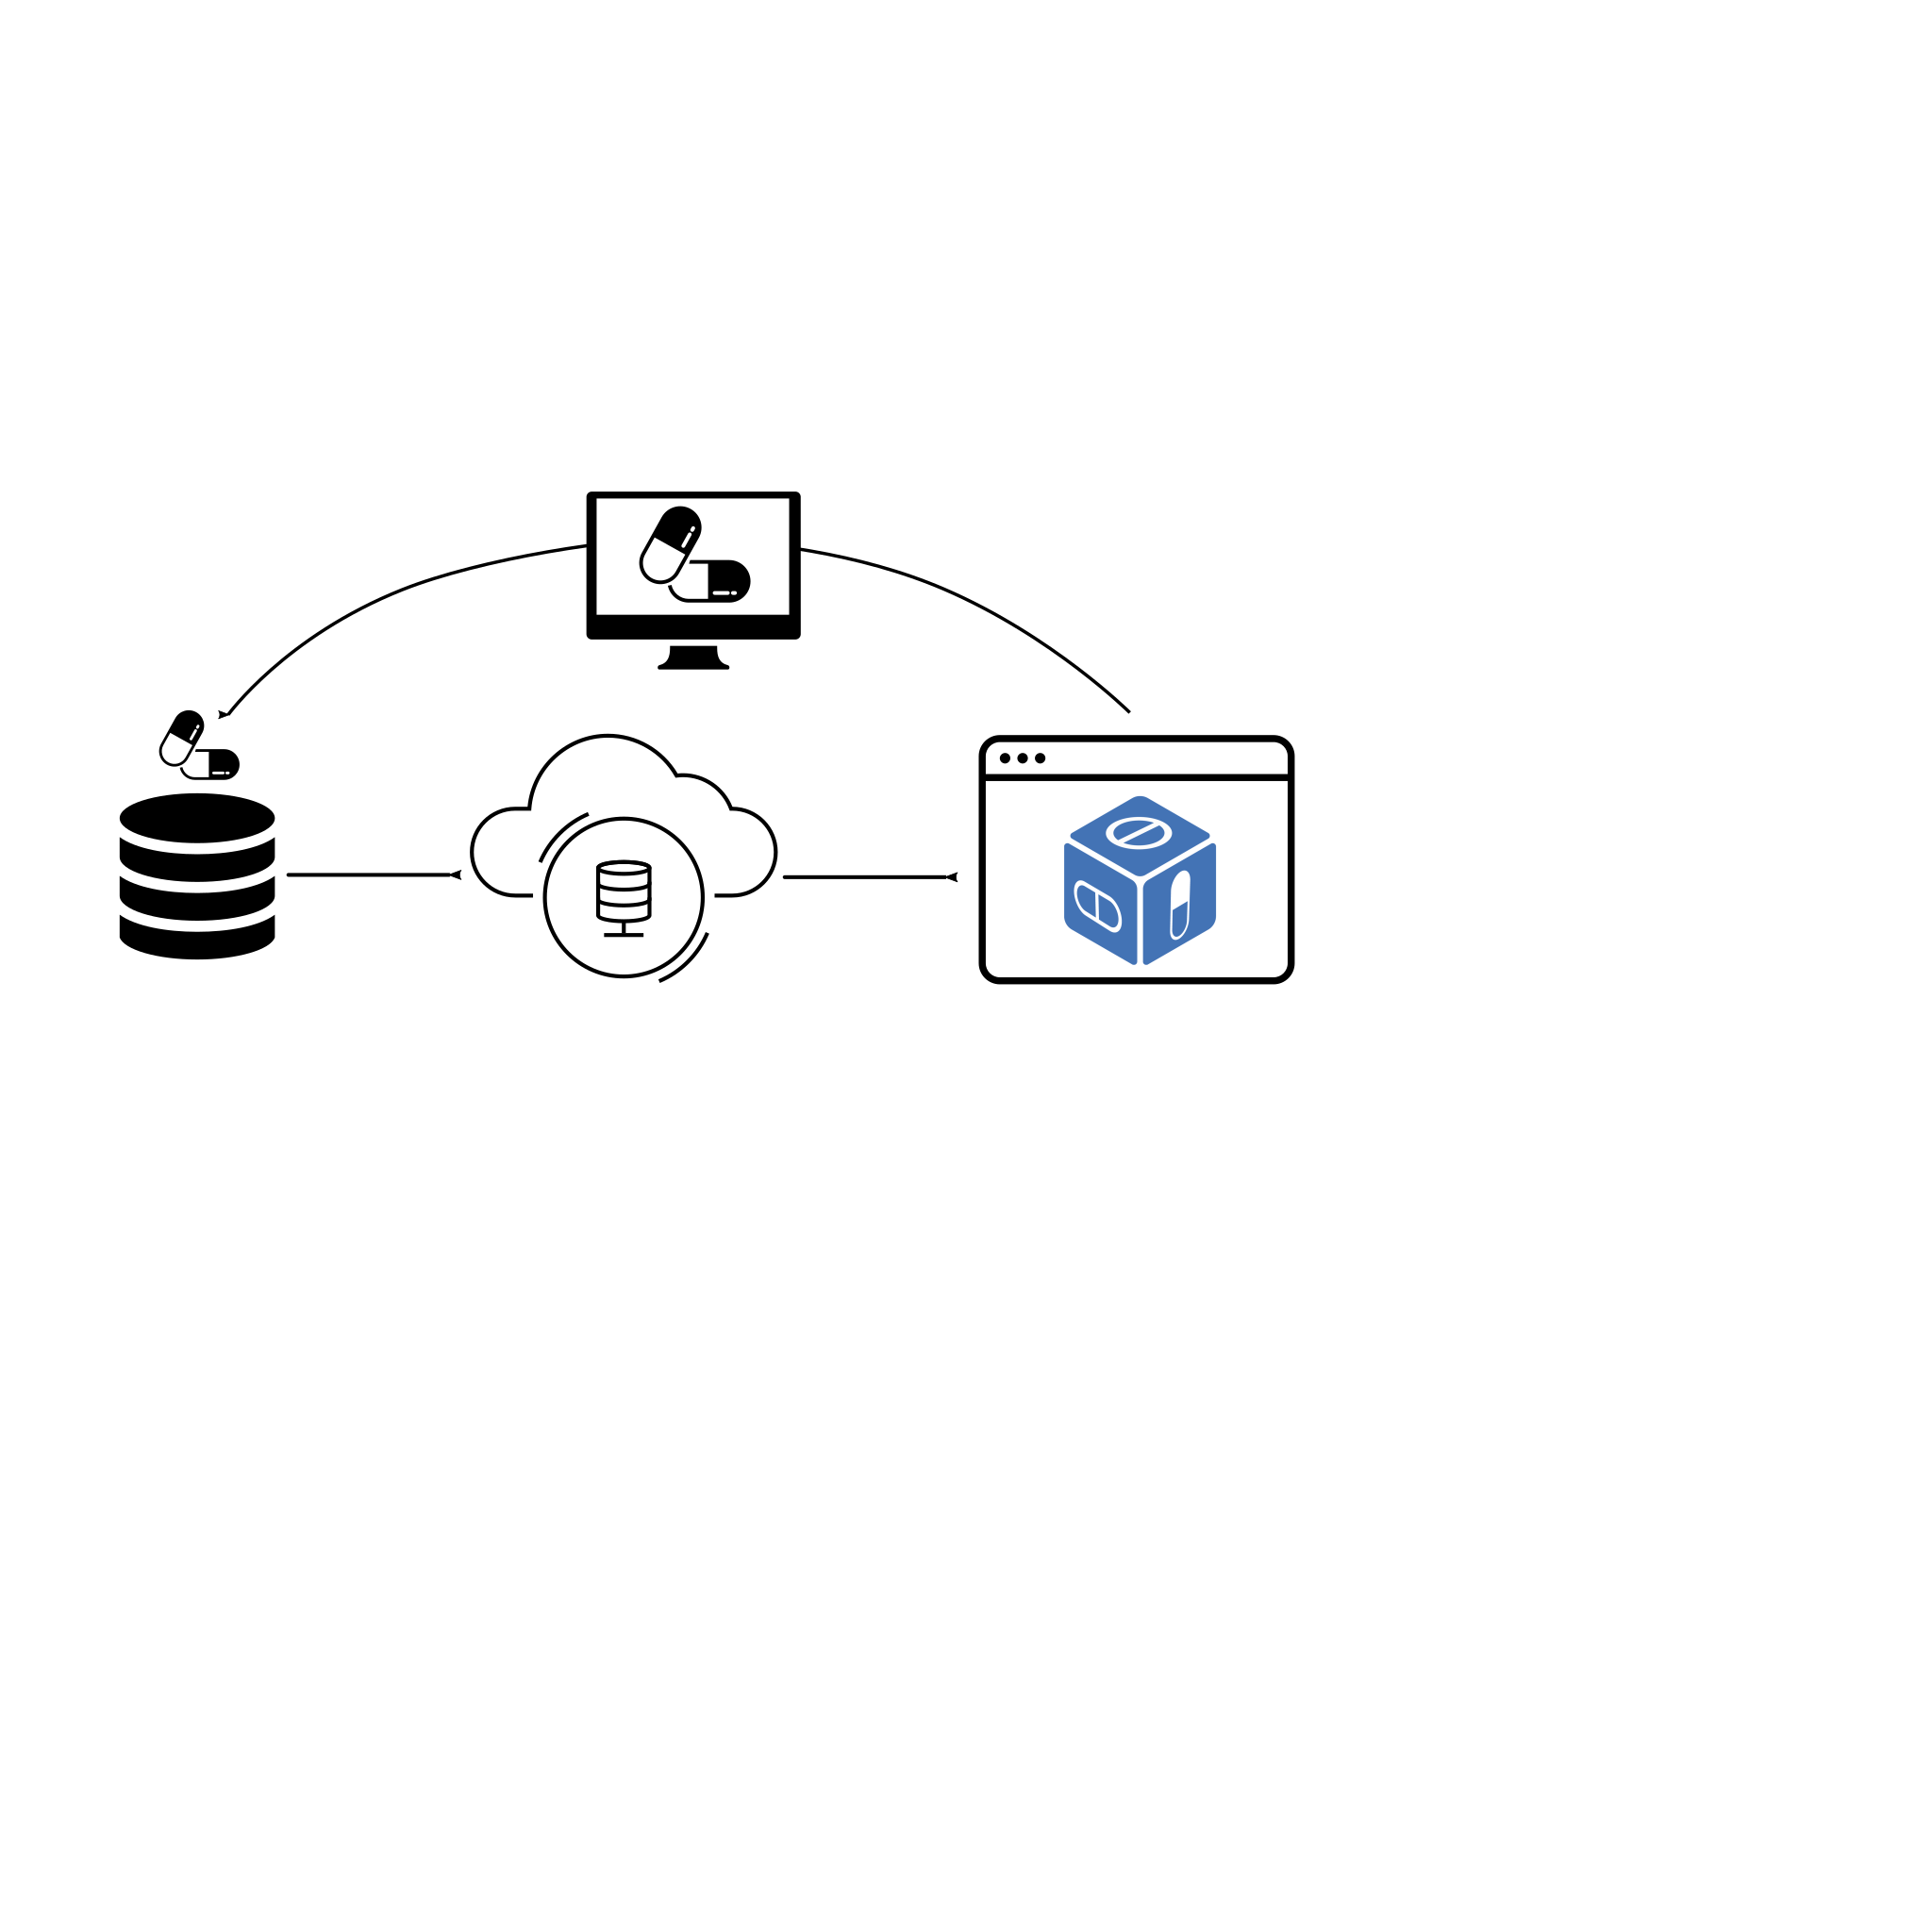
\includegraphics[width=0.9\textwidth]{workflow}}
\caption{A diagram representation of the computational infrastructure
  presented. Spontaneous reporting system data is processed on grid
  computing systems to generate an adverse event database with a web
  front-end which has an on-demand interface to request drug
  combination adverse reactions. }
\label{fig:workflow}
\end{figure}

A key feature of the computing infrastructure presented is portability
to other spontaneous reporting systems, such as EudraVigilance.  This
allows researchers to create their own version of the back-end
database for any use, including incorporation into the nSides web
gateway. Additionally, using consistent algorithms across
spontaneous reporting systems allows researchers to evaluate drug
effect differences and bias due to drug approval process differences.

The computational infrastructure with instructions can be found on
GitHub, at https://github.com/tatonetti-lab/nsides.


\section{Data Sources}

We built nSides using several data sources. We use a
curated version of the FDA Adverse Event Reporting System (FAERS)
known as Adverse Event Open Learning through Universal Standardization
(AEOLUS)~\cite{AEOLUS}.  AEOLUS aims to clean and normalize the data
by removing duplicate cases. This is done by mapping drug names to RxNorm and outcomes to SNOMED-CT---two standardized vocabularies that are widely accepted in informatics. The AEOLUS dataset is publicly available.

Using standard vocabularies for drug names and outcomes allows
other spontaneous reporting systems to be adapted to a consistent
format used on the AEOLUS dataset. Furthermore, this strategy facilitates
semantic interoperability with other informatics tools, allowing nSides to be
more easily incorporated into complex workflows and analysis pipelines.

\section{Methods}
In this paper, we focus on the distributed computing setup used to learn and visualize the results of nSides. Before describing this setup, we will briefly describe the algorithmic approach used to learn the nSides database.

\subsection{Adverse Event Detection Algorithm}
The algorithm used to develop the databases comprising nSides is an
updated version of the one used to populate the O\textsc{ffsides} and
T\textsc{wosides} databases.  These databases contain side effect
significances calculated using raw FAERS data~\cite{Tatonetti2012}.
Generally, a standard signal detection algorithm involves conducting a
disproportionality analysis by comparing the observed reporting
frequency of a drug and outcome to the expected reporting frequency of
all other drugs and the outcome. The metric is known as a Proportional
Reporting Ratio (PRR). If the outcome occurred by chance, the
frequencies will be equal and the PRR will be one. If the PRR is
significantly greater than one, the null hypothesis is rejected. To
reduce sampling variance and selection bias, propensity score matching
is implemented to form the groups used in the disproportionality
analysis. This procedure, known as SCRUB, matches cases and controls
between patients exposed and not exposed to a particular drug
(O\textsc{ffsides}) or two drugs (T\textsc{wosides}) to mitigate
confounding biases. Once cases and controls are matched, the PRR for
various side effects are calculated. An example is shown in
Fig.~\ref{fig:prr}.

\begin{figure}[h]
\centerline{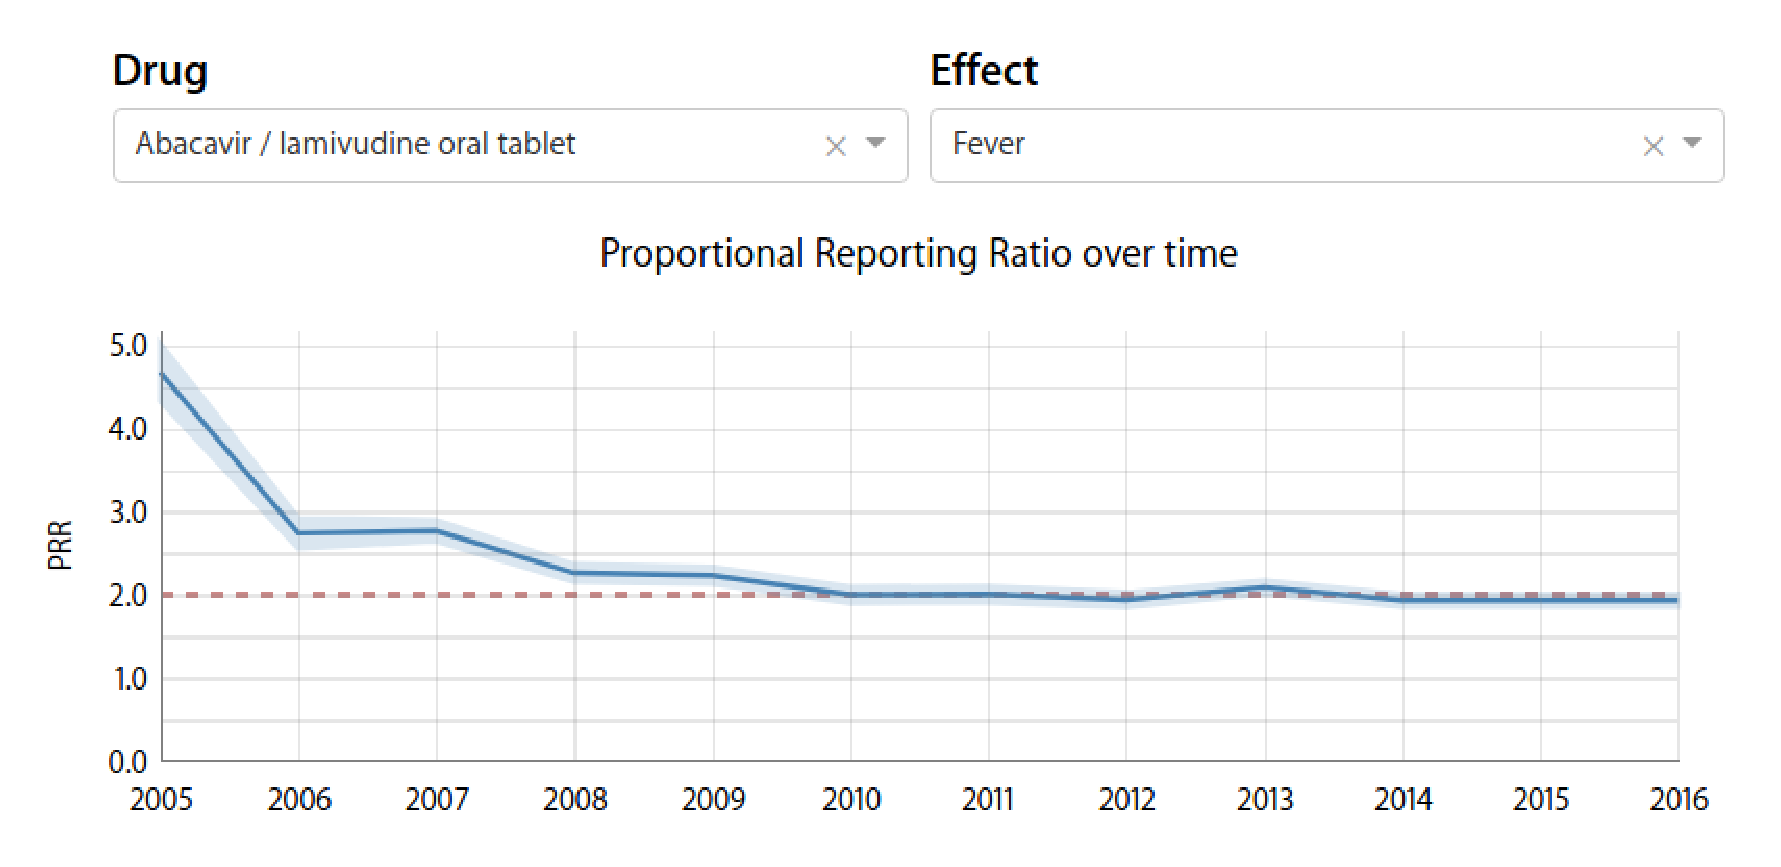
\includegraphics[width=0.7\textwidth]{prr}}
\caption{Example result using the nSides front-end web gateway. Shown
  is PRR calculated from the reports taken up to the year on the
  x-axis.}
\label{fig:prr}
\end{figure}

There are several key differences between the O\textsc{ffsides} and
T\textsc{wosides} databases and nSides. The updated algorithm uses a
deep learning model as well as logistic regression to calculate
propensity scores to match cases and controls. By using two algorithms
instead of just one, and the increased complexity of deep learning
models, the computational power required to populate the nSides
back-end database is much greater. Since nSides is not designed to be
limited to effects of single and interactions of two drugs, a much
more robust computational infrastructure is required.

\subsection{Computational Challenge}

Populating the nSides database requires the SCRUB procedure to be run
for each drug or combination of drugs individually to identify
appropriate cases and controls. Once we have identified cases and
controls, we then needed to calculate PRR values over a range of side
effects. Since the AEOLUS dataset contains $\approx$4,000 drugs,
$\approx$5,000,000 reports, and $\approx$8,000 effects to analyze, a
computational challenge emerges.  To deal with this challenge, we
employ resources made available by the Open Science Grid (OSG) and
Columbia University's computing cluster, Habanero. The OSG provides
access to computing resources for research in the United States, free
of charge. The computing facilities are located at over 100 sites
spanning the United States, primarily at universities and national
laboratories. The computing infrastructure we present is optimized to
work on the OSG to increase the portability of the infrastructure to
other spontaneous reporting systems, but our use of Habanero
demostrates that it can be easily adapted to other distributed
computing platforms as well.

Initially, we populate the nSides database with single drug
effects. To do this, we learn a deep neural network model and a
logistic regression model for each of the $\approx$4,500 unique drugs
in the AEOLUS dataset. We learn the models using the two scientific
computing libraries TensorFlow and scikit-learn, respectively. The
computation involved in generating the deep neural network model is
more intensive than that of the more traditional logistic regression
model, such as those used in the creation of O\textsc{ffsides} and
T\textsc{wosides}. As a result, we found it necessary to construct a
more robust computational infrastructure.

As mentioned previously, the task of fully populating the back-end
database for multiple drug interactions quickly becomes
intractable. We show how the number of models to compute for the
interaction of two and three drugs scales with the number of total
drugs in Fig.~\ref{fig:drug_interactions}.

TODO: Figure with number of drugs (x-axis) and number of models that need to be computed (y-axis)

\subsubsection{Distributed Computing Strategy}
The combinatorial complexity of running all jobs scales on the order
of $\Theta(N^2)$ in the number of drugs. Given that a single job
running on an OSG node takes 4-10 hours to complete, a distributing
computing strategy is necessary to make the total runtime
practical. As mentioned above, we utilized two distributed computing systems to determine
the PRR between all pairs of coreported drugs.

The first of these was provided by the OSG. The OSG uses the HTCondor job submission
software~\cite{beowulfbook-condor}, which handles allocation of
computing resources to jobs submitted by the user. The other
distributed computing system we utilized was Columbia University's
scientific computing cluster, named Habanero. Habanero, like the OSG,
uses a job submission management system, but unlike the OSG, Habanero
uses the Slurm workload manager~\cite{slurm} for user-submitted
jobs. We used both HTCondor and Slurm to submit jobs in a directed
acyclic graph (DAG) configuration, supported using native extensions
to HTCondor and Slurm~\cite{dagman}. In short, the DAG strategy allows
users to take advantage of the fact that many distributed computing
workflows consist of jobs containing common elements, such as initial
data preparation. In a simplified example, a workflow may consist of
one invariant data preparation stage followed by two sequential
machine learning models, where each step relies on the previous step,
and the machine learning models accept variable parameters. Here, the
DAG capabilities of HTCondor and Slurm will only run the first stage
one time, and sequentially pass the results of each stage to the next
stage with the appropriate parameters, as the results of the previous
stage are available. This approach allows us to substantially reduce
the combinatorial complexity of running all jobs to a manageable
level.

Since HTCondor and SLURM are two very common job schedulers, we
release code such that the nSides back-end infrastructure can be
easily deployed on either, which increases the portability of
the infrastructure to other spontaneous reporting systems.

\subsection{Computational Structure}
Generating a model for an individual drug or drug combination involves the following:

\begin{enumerate}
\item {\it Data preparation}: Dimensional reduction of the complete AEOLUS dataset to reduce computational complexity of generating models. To do this, we only consider co-reported drugs that appear in at least 1 report
\item {\it Model generation}: Generate 20 deep learning and logistic regression models per drug using different subsets of exposed and non-exposed reports. This is done to increase generality of the model.
\item {\it Model evaluation}: Use scores generated by models to perform propensity score matching, use propensity score matched cases and controls to calculate side effect PRR values. For comparison, PRR values are also generated without propensity score matching.
\item Populate nSides back-end MongoDB database.
\end{enumerate}

Steps (1) through (3) are performed in a grid computing environment in
with the DAG strategy, shown in Fig.~\ref{fig:dag}.  Step (4) is
dependent on the hosting structure of the MongoDB back-end.

\begin{figure}[h]
\centerline{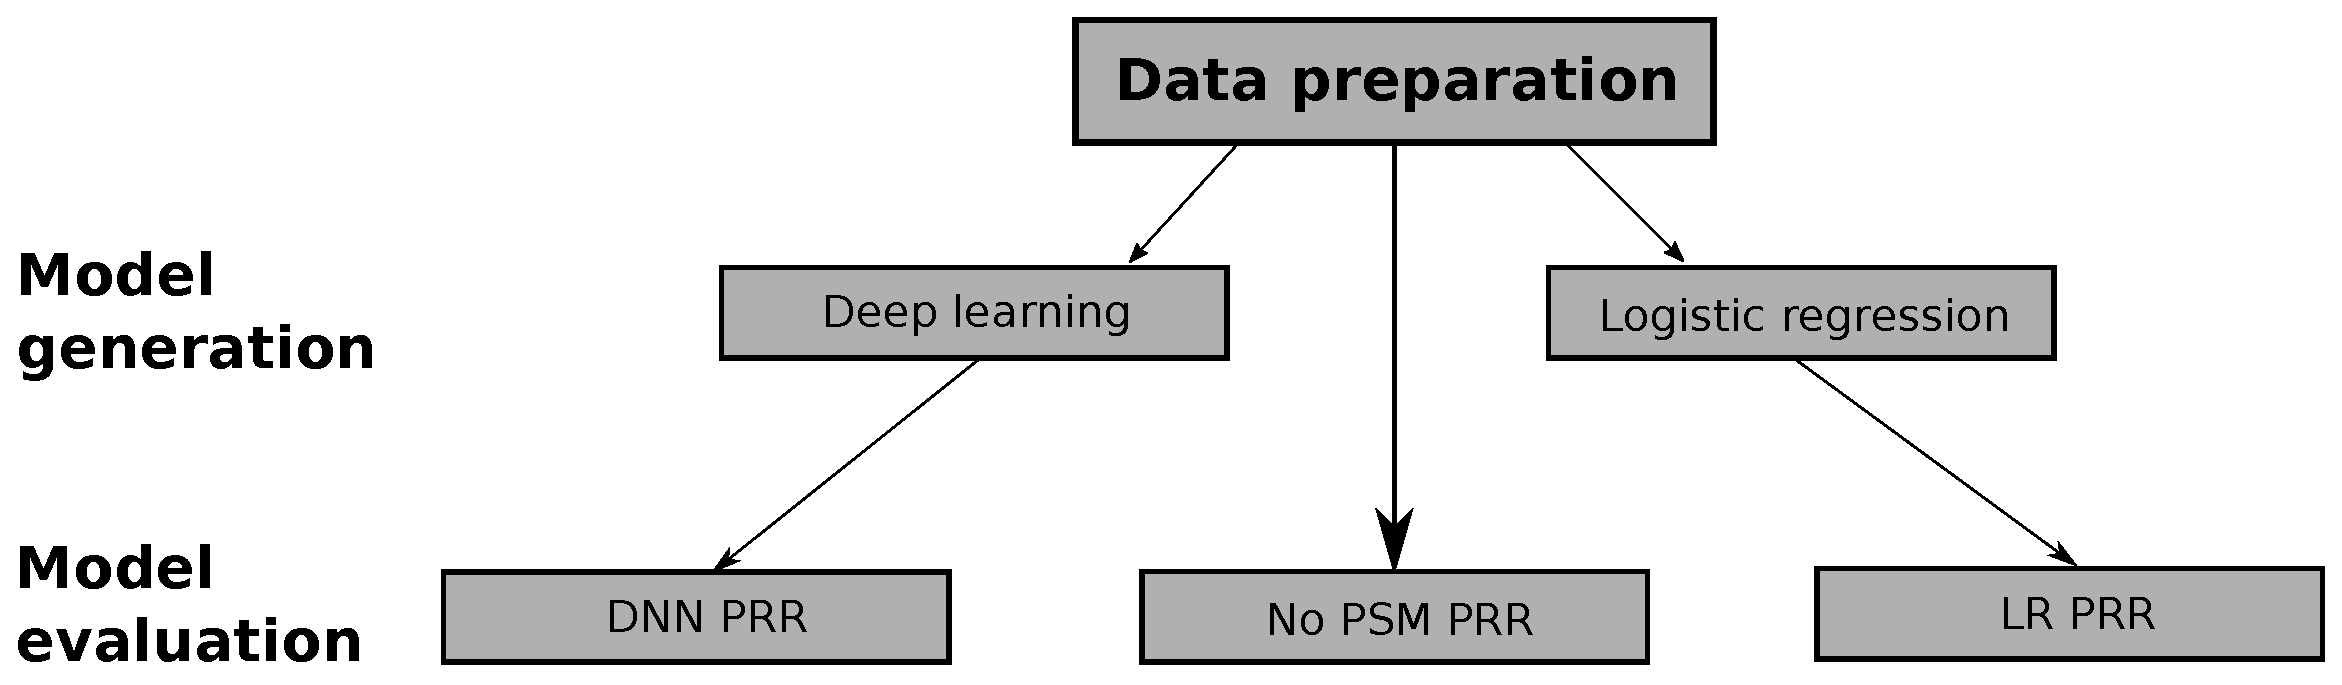
\includegraphics[width=\textwidth]{dag}}
\caption{Computational structure employed on distributed computing
  systems. First the data for a particular drug or drug combination is
  pre-processed, then 20 deep learning and logistic regression models
  are generated for that specific drug or drug combination and finally
  propensity score matching is performed to result in PRR values.}
\label{fig:dag}
\end{figure}


\subsection{On-demand Interface}
We originally performed testing of our methods manually on the two
distributed computing servers using a command line interface and shell
scripts. In order to improve the ease of job submission in the future,
we have developed a robust searchable shared-usage gateway to the OSG
resources we have described previously. The gateway uses a
three-tiered architecture consisting of browser-based user interfaces
on the frontend, the OSG job submission system on the backend, and
middleware to facilitate communication between the other two
components. We deploy the user interfaces using an application written
using the Python Flask framework, which then access a variety of web
services that constitute the middle tier of the gateway. These web
services are arranged in a way that allows a heterogeneous collection
of resources to be accessed remotely in a uniform fashion.

Additionally, we have bundled the user interface frontend alongside a
RESTful Web API (Application Programming Interface) that allows
authenticated users to submit jobs programmatically. This API is
implemented using the Agave tenant service~\cite{dooley2012agave}---a
cloud-based API system designed for developing APIs to be used for
scientific computing. The Agave job API manages all aspects of job
execution and management, including data staging, job submission, job
monitoring, output archiving, event logging, sharing, and
notifications.

\section{Discussion}

Creating an open-source computing infrastructure for mining and
presenting side effect significances from spontaneous reporting
systems has great potential for improving pharmacovigilance. By using
the same algorithm across many systems, we have demonstrated that it
is possible to evaluate drug effect significance differences which can
be used to reduce the potential of adverse drug effects.

Due to dataset restrictions, it is not always possible to incorporate
spontaneous reporting system data other than FAERS directly. For
example, EudraVigilance data is only available to academic
institutions within the European Union. Using our infrastructure, it
is possible for researchers with access to EudraVigilance to form a
separate version of nSides which can be compared to the version made
with FAERS data.

\section{Acknowledgements}
R.S.V., J.D.R., T.L., V.N., and N.P.T. are supported by grants from
the National Institutes of Health, NIGMS R01GM107145 and NCATS
OT3TR002027. R.S.V. and N.P.T. are also supported by the Herbert
Irving Fellowship. This research is done using resources provided by
the Open Science Grid~\cite{pordes2007open, sfiligoi2009pilot}, which
is supported by the National Science Foundation award 1148698, and the
U.S. Department of Energy's Office of Science.  This research is also
supported by the Science Gateways Community Institute's Extended
Developer Support program, funded by the National Science Foundation
award 1547611.





\bibliographystyle{ws-procs11x85}
\bibliography{ws-pro-sample}

\end{document}
